%AGREGAR:
%fotos, graficos
%explicar y mostrar simulaciones
%comparar para el noise margin la simulacion con las distintas R
%lo del capacitor de 1 nF

%\documentclass[a4paper,11pt]{report}
%
%\usepackage[options]{package}
%\usepackage{graphicx}
%\usepackage{color} 
%\usepackage[dvipsnames]{xcolor}
%\colorlet{purple}{purple}
%\usepackage{textgreek}

%%% Preamble
\documentclass[paper=a4,fontsize=11pt]{report}


\begin{document}

\section{\color{olive}Exercise 1: Design and Implementation of NOT Gates Using Transistors} %Despues borrar el Exercise 1 del titulo y que queden solo los titulos de los ejs en color olive.

The following parameters are important when designing NOT Gates.

\subsubsection{\color{red}High-Level and Low-Level Input Voltages}
The high-level input voltage ($V_{IH}$) is the minimum input voltage that is considered as high, while the low-level input voltage ($V_{IL}$)  is the maximum input voltage that is considered as low.

\subsubsection{\color{red}High-Level and Low-Level Output Voltages}
The high-level output voltage ($V_{OH}$) is the minimum output voltage that the circuit provides as a high, while the low-level output voltage ($V_{OL}$) is the maximum output voltage that the circuit provides as a low.

\subsubsection{\color{red}Noise Margin}
The high noise margin ($NM_{H}$) is the gap between the high-level input voltage and the high-level output voltage, while the low noise margin ($NM_{L}$) is the gap between the low-level output voltage and the low-level input voltage.
$$NM_{H} = V_{OH} - V_{IH}$$
$$NM_{L} = V_{IL} - V_{OL}$$

\subsubsection{\color{red}Propagation Delays}
For this assignment's meassures, when the input changes from low to hight and the output from high to low, the high-to-low propagation delay is considered as the time between the moment in which the input voltage reaches the $90\% $ of its maximum high value, until the moment in which the output voltage reaches the $10\%$ of its maximum high value.
$$t_{pHL} = t_{10\%V_{maxO}} - t_{90\%V_{maxI}}$$
In the case in which the input goes from high to low and the output from low to high, the low-to-high propagation delay is considered as the time between the moment in which the input voltage reaches the $10\%$ of its maximum high value, until the moment in which the output voltage reaches the $90\%$ of its maximum high value.
$$t_{pLH} = t_{90\%V_{maxO}} - t_{10\%V_{maxI}}$$

\subsubsection{\color{red}Transition Times}
The high-to-low transition time or fall time ($t_{f}$) is the time that it takes the output voltage to go from its high maximum value to its low minimum value, while the low-to-high transition time or rise time ($t_{r}$) is the time that it takes for it to change from its low minimum value to tis high maximum value.


\subsubsection {\color{red}Maximum Output Current}
The maximum output current the circuit provides in the output, which will take place when there is a capacitor, is calculated from the equation:
$${I_C}=C\frac{dVc}{dt}$$
Where the maximum output current of the circuit will take place when there is a change in the voltage, form high to low or low to high. 

ESTO ES NPN PARA MAX CURRENT
\begin{figure}[h!]
\centering
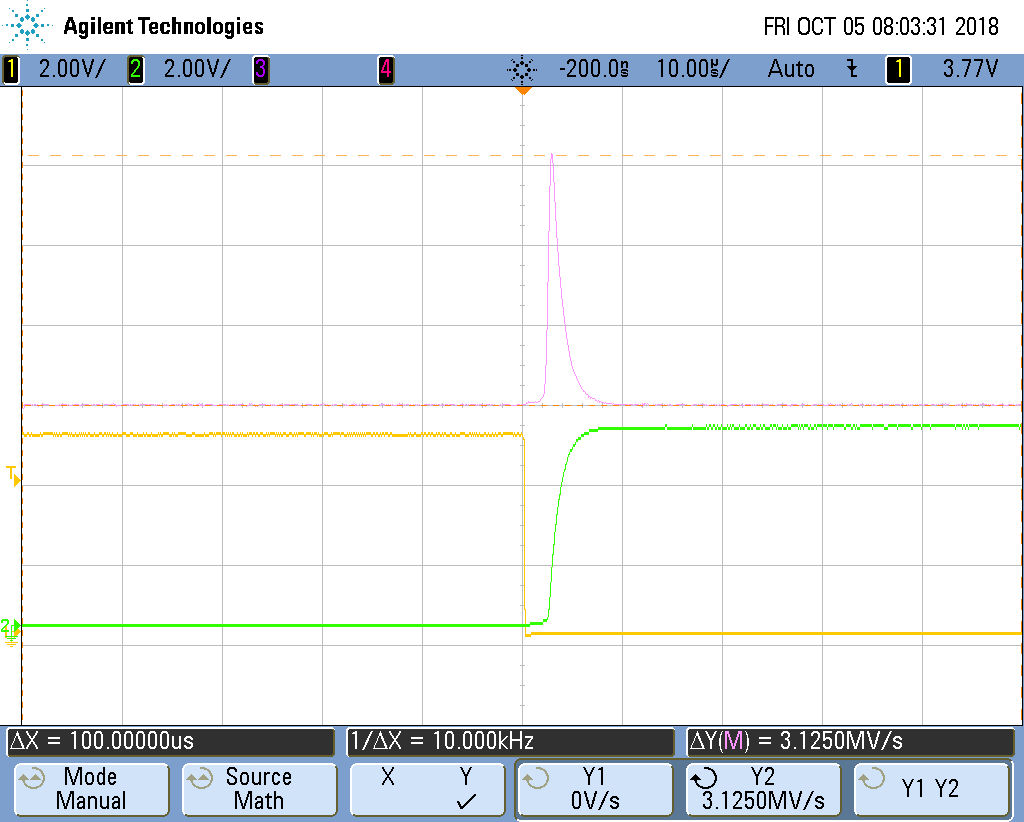
\includegraphics[scale=0.3]{../Exercise1/i_npn2.png}\hspace{1cm}
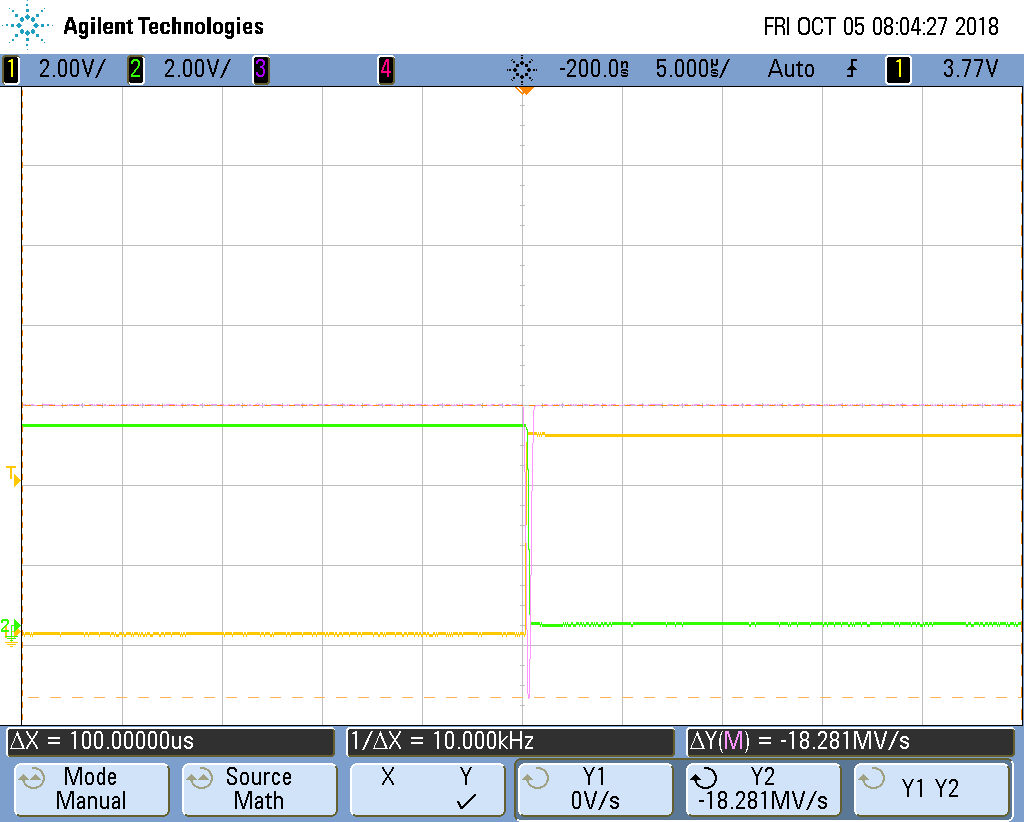
\includegraphics[scale=0.3]{../Exercise1/i_npn3.png}
\caption{NPN Maximun output current}
\label{circnpnmaxout}
\end{figure}

ESTO ES PNP PARA MAX CURRENT
\begin{figure}[h!]
\centering
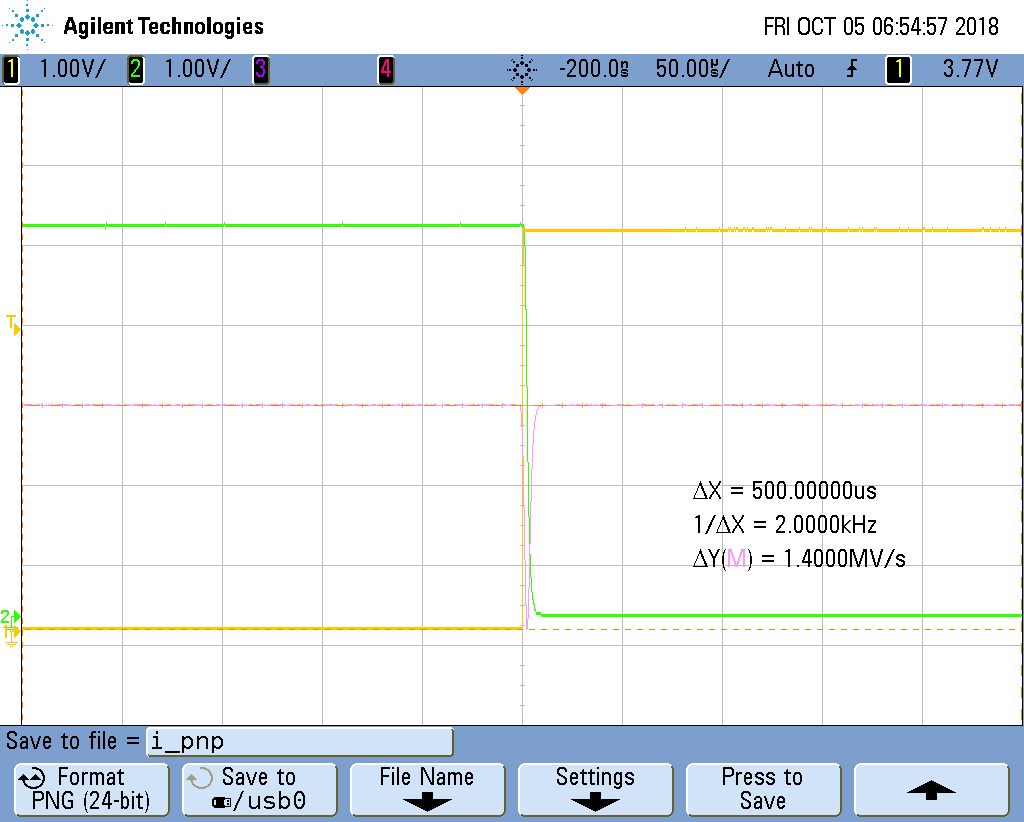
\includegraphics[scale=0.3]{../Exercise1/i_pnp.png}\hspace{1cm}
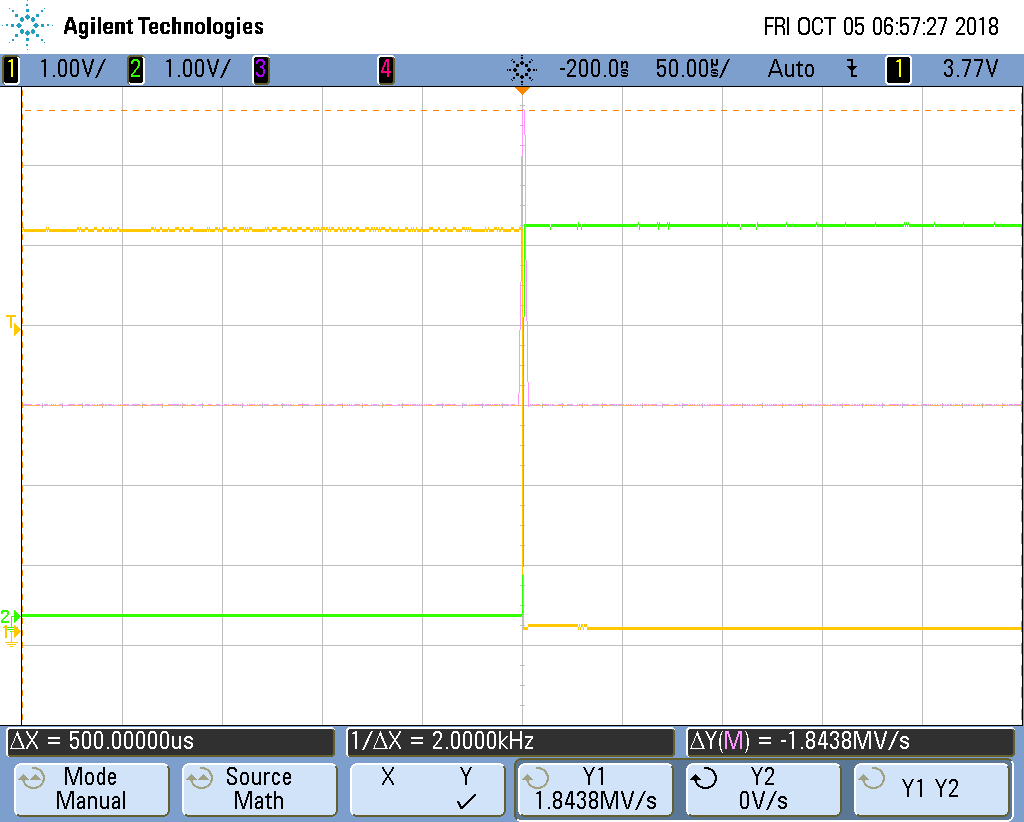
\includegraphics[scale=0.3]{../Exercise1/i_pnp1.png}
\caption{PNP Maximun output current}
\label{circpnpmaxout}
\end{figure}


\subsection{\color{purple}NOT Gates' Designs}

\begin{figure}[h!]
\centering
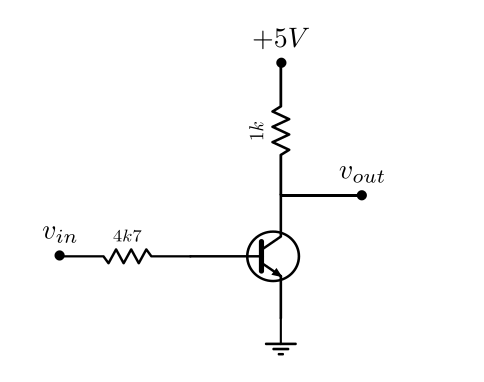
\includegraphics[scale=1]{../Exercise1/circuitoNPN}
\caption{NOT Gate Using a NPN Transistor}
\label{circNPN}
\end{figure}

\begin{figure}[h!]
\centering
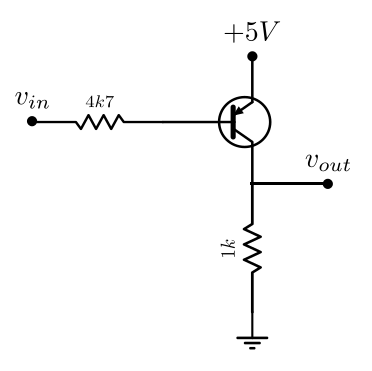
\includegraphics[scale=1]{../Exercise1/circuitoPNP}
\caption{NOT Gate Using a PNP Transistor}
\label{circPNP}
\end{figure}
%ESCRIBIR ACA LO DE LA DERIVADA DE LA TENSION EN EL OSCILOSCOPIO

<<<<<<< Updated upstream
Figure \ref{circPNP} represents a NOT gate built with a BJT NPN 337 transistor, while the circuit in Figure \ref{circPNP} corresponds to a NOT gate that uses a BJT PNP 327 transistor. The $4,7k{\Omega}$ resistors that appear in both circuits where chosen after simulations made with LTspice. We evaluated how the noise margin changed according to this resistor's value. As it is preffered to have a small noise margin because it corresponds to the "prohibited" voltage values, the $4,7k{\Omega}$ resistor was chosen over bigger values.



 %mostrar simulaciones ACA (HACER DENUEVO LA DE 47K)

\subsection{\color{purple}Measurements}

The parameters defined above were measured for each of the circuits in Figures \ref{circNPN} and \ref{circPNP} in two different conditions: without loading the output and with a $1 nF$ capacitor connected to the output. Te results are shown in the following table. \\
=======
\subsection{\color{purple}Measurements}


\subsection{\color{purple}Using a BJT NPN 337 Transistor}

\subsubsection{\color{red}Without Load Connected to the Output}

\subsubsection{\color{red}With a $1 nF$ Capacitor Connected to the Output}


\subsection{\color{purple}Using a BJT PNP 327 Transistor}

\subsubsection{\color{red}Without Load Connected to the Output}

>>>>>>> Stashed changes

\begin{tabular}{|c|c|c|c|c|}
\hline
 & NPN & NPN with capacitor &PNP& PNP with capacitor\\
\hline
\hline
$V_{IH} (V)$ & 0,9 & 0,9 & 4,5 & 4,6  \\
\hline
$V_{IL} (V)$ & 0,5V & 0,6 & 4,2 & 4,3 \\
\hline
$V_{OH} (V)$ & 4,96V & 4,56 & 4,77 & 5 \\
\hline
$V_{OL} (V)$ & 0,1 & 0,12 & 0,05 & 0,45\\ 
\hline
$NM_{H} (V) $ & 4,06 & 3,66 & 0,27 & 0,4\\ %se pone en VOLTS???????????????????????????
\hline
$NM_{L} (V) $ & 0,4 & 0,48 & 4,15 & 3,85 \\  %se pone en VOLTS???????????????????????????
\hline
$t_{pHL}$ & 87ns & $2,7\mu s $ &  $2,72\mu s$ & 101ns \\
\hline
$t_{pLH}$ & $2,94\mu s$ &  104ns &  73ns &  $2,23\mu s$\\
\hline
$t_{f}$ & 69,5ns & 84ns & 575ns & 770ns\\
\hline
$t_{r}$ & 505ns & 520ns & 83ns & 86 ns\\
\hline
$ I_{Out{Max}}$ &   &   &   &   \\ %AGREGAAAAAAAAAAAAAAAAAAAR
\hline
\end{tabular}





\end{document} 
























